\documentclass[12pt]{article}

% Encoding for document, allows for use of characters beyond ASCII
\usepackage[utf8]{inputenc}

% Math symbols
\usepackage{amsmath}

% Change margins
\usepackage[margin=1in]{geometry}

% Control page headers and footers
\usepackage{fancyhdr}
\pagestyle{fancy}

% Change text colors
\usepackage[dvipsnames,table]{xcolor}

% Produce hypertext links in the document
\usepackage{hyperref}

%Write Chemical Equations: 
\usepackage{mhchem}

%Bibliography Resources
\usepackage[sorting = none]{biblatex}
\addbibresource{references.bib}

% Set the default indentation to be none
\setlength\parindent{0pt}

% Wrap text around figure 
\usepackage{wrapfig}

\usepackage{verbatim,graphicx,amsmath,amssymb,mathrsfs,mathtools,dsfont,mathabx,dcolumn,amsthm,enumitem,commath,physics}
\usepackage{pgfplots}
\usepackage{float}
\usepackage{tikz}
\usepackage{listings}
\usepackage{color}
\usepackage{subcaption, appendix, cancel}
\newcommand{\iu}{{i\mkern1mu}}

\definecolor{mygreen}{rgb}{0,0.6,0}
\definecolor{mygray}{rgb}{0.5,0.5,0.5}
\definecolor{mymauve}{rgb}{0.58,0,0.82}

\lstset{ 
  backgroundcolor=\color{white},   % choose the background color; you must add \usepackage{color} or \usepackage{xcolor}; should come as last argument
  basicstyle=\footnotesize,        % the size of the fonts that are used for the code
  breakatwhitespace=false,         % sets if automatic breaks should only happen at whitespace
  breaklines=true,                 % sets automatic line breaking
  captionpos=b,                    % sets the caption-position to bottom
  commentstyle=\color{mygreen},    % comment style
  deletekeywords={...},            % if you want to delete keywords from the given language
  escapeinside={\%*}{*)},          % if you want to add LaTeX within your code
  extendedchars=true,              % lets you use non-ASCII characters; for 8-bits encodings only, does not work with UTF-8
  firstnumber=1,                % start line enumeration with line 1000
  frame=single,	                   % adds a frame around the code
  keepspaces=true,                 % keeps spaces in text, useful for keeping indentation of code (possibly needs columns=flexible)
  keywordstyle=\color{blue},       % keyword style
  language=Matlab,                 % the language of the code
  morekeywords={*,...},            % if you want to add more keywords to the set
  numbers=left,                    % where to put the line-numbers; possible values are (none, left, right)
  numbersep=5pt,                   % how far the line-numbers are from the code
  numberstyle=\tiny\color{mygray}, % the style that is used for the line-numbers
  rulecolor=\color{black},         % if not set, the frame-color may be changed on line-breaks within not-black text (e.g. comments (green here))
  showspaces=false,                % show spaces everywhere adding particular underscores; it overrides 'showstringspaces'
  showstringspaces=false,          % underline spaces within strings only
  showtabs=false,                  % show tabs within strings adding particular underscores
  stepnumber=2,                    % the step between two line-numbers. If it's 1, each line will be numbered
  stringstyle=\color{mymauve},     % string literal style
  tabsize=2,	                   % sets default tabsize to 2 spaces
  title=\lstname                   % show the filename of files included with \lstinputlisting; also try caption instead of title
}
% Set the header 
\lhead{Jonathan H. Vo} % Left header (Name and Student ID Number)
\chead{\textbf{\large Mathematical Model Draft}} % Center header (Title)
\rhead{Lowengrub Lab \\ \today} % Right header (Class Name & today's date)

%%%%%%%%%%%%%%%%%%%%%%% Begin Document %%%%%%%%%%%%%%%%%%%%%%% 
%\title{Template}
%\author{Jonathan Vo}
%\date{\today}
\setlength{\parindent}{0.0in}
\setlength{\parskip}{0.05in}
\begin{document}
%\maketitle
\section*{Yu model}
Victoria Yu's model is as follows:
\begin{align*}
\dv{\hat{U}}{t} &= (2p-1)k(\hat{W})r_1\hat{U}\\
\dv{\hat{V}}{t} &= 2(1-p)k(\hat{W})r_1\hat{U} + (r_2k(W)-d)\hat{V},
\end{align*}
where $\hat{W}=\hat{U}+\hat{V}$, $k(\hat{W})=1-\hat{W}^4$, and $\hat{U}$ and $\hat{V}$ are volume fractions of the tumor volume
LQ model:
\begin{align*}
\hat{U}_s &= \hat{U}\cdot e^{-\alpha_{\hat{\text{U}}}{d_i}-\beta_{\hat{\text{U}}}{d_i}^2} + c\cdot d_i\cdot \hat{V}\\
\hat{V}_s &= \hat{V}\cdot e^{-\alpha_{\hat{
\text{V}}}{d_i}-\beta_{\hat{\text{V}}}{d_i}^2}
 - c\cdot d_i\cdot \hat{V}
\end{align*}
\section*{Kim model}
Nayeon Kim's model is as follows:
\begin{align*}
\dv{U}{t} &= \left(2p-1\right)\cdot r_1\cdot U\\
\dv{V}{t}&=2\left(1-p\right)\cdot r_1\cdot U+(r_2-d)V,
\end{align*}
where $U = \left(\frac{1}{\rho}N\right)\hat{U}$, $V = \left(\frac{1}{\rho}N\right)\,\hat{V}$, $p\leftarrow \frac{\bar{p}}{1+l\,V^n},r_1\leftarrow \frac{\bar{r_1}}{1+h\,V^z},r_2\leftarrow \frac{\bar{r_2}}{1+h\,V^z}$ This rescaling allows us to translate results between models, which only differ in how rate parameters are controlled. In Yu's model, a logistic type of growth controls the division rates. Meanwhile, Kim's model uses negative feedback from differentiated cells on division rate and on probability of proliferation, and we assume the same feedback takes place on both division rates.


The LQ model followed exactly from that of Yu  up to that factor of conversion between volume and cell number: 
\begin{align*}
U_s &= U\cdot e^{-\alpha_{\text{U}}{d_i}-\beta_{\text{U}}{d_i}^2}+c\cdot d_i\cdot V\\
V_s &= V\cdot e^{-\alpha_{
\text{V}}{d_i}-\beta_{\text{V}}{d_i}^2} - c\cdot d_i\cdot V
\end{align*}
%\section*{Moving to a new model}
%In order to study the effect of survivin and chemotherapy on tumor survival after therapeutic interventions take place, we have apoptosis of differentiated cells be subject to negative feedback from itself as a proxy for survivin in the interim. An additional extension to Kim's model is that survivin has a rate equation and that the reprogramming term of the LQ model is restricted to having a maximum value of 1, as we should not allow the model to get more differentiated cells than is physically possible. A further modification is to have only differentiated cells which survive radiotherapy to reprogram.
\section*{Moving to a new model}
\begin{itemize}
\item In order to study the effect of survivin and chemotherapy on tumor survival after therapeutic interventions take place, we have apoptosis of differentiated cells be subject to negative feedback from itself as a proxy for survivin in the interim.
\item An additional extension to Kim's model is that survivin has a rate equation and that the reprogramming term of the LQ model is restricted to having a maximum value of 1, as we should not allow the model to get more differentiated cells than is physically possible.
\item A further modification is to have only differentiated cells which survive radiotherapy to reprogram.
%\item Following Yu and Hillen (2013), tumor is with cell density $10^9$ into a spheroid of 1 unit of radius (a millimeter?)
%\item We interpret $U$ and $V$ as being volume fraction of stem cell and terminally differentiated cell. %We interpret $U$ and $V$ as being density of stem cell and terminally differentiated cell. Given the prior assumption, we can re-interpret $U$ and $V$ as number of cells per Kim's thesis. If we assume finite size of the cells, then we can re-interpret $U$ and $V$ as being volume fractions, per Yu's thesis. Thus we can readily achieve equivalency of the three measures of abundance of cell used for this sort of lineage model at the multiplication of the appropriate constant. 
%\item Initial fraction of maximum tumor size at $t_0$ is $\frac{0.2}{64}$.
\item Extracellular survivin amounts produced from the cell are not negligible during normal tumor growth; in fact, survivin is constitutively secreted in normal and cancer cells. However, for now we ignore it to study the effects of radiotherapy on survivin alone. We expect results to indicate less pronounced recurrence of tumor.
\item Effects of survivin on apoptosis will be only temporarily ignored, as we want to study the effects of survivin on radiotherapy alone. We expect results to possess a further reduced rate of growth in the tumor. Specifically, there will be fewer stem cells and fewer differentiated cells than expected. Either by measurement or by literature search can parameters relevant to this limitation or the one before be used to relax them.
\end{itemize}

\section*{Survivin model 1}
\subsection*{Tumor Growth}
\begin{align*}
\dv{U}{t}&=\left(2p-1\right)\cdot r_1\cdot U\\
\dv{V}{t}&=2\left(1-p\right)\cdot r_1\cdot U +(r_2-d)V\\
\dv{S}{t}&=-\sigma S,
\end{align*}
\[p\leftarrow\frac{\bar{p}}{1+l\,V^n},r_!\leftarrow\frac{\bar{r_1}}{1+h\,V^z},r_2\leftarrow\frac{\bar{r_2}}{1+h\,V^z},d\leftarrow\frac{\bar{d}}{1+h\,V^z}\]
\subsection*{Radiotherapy}
\begin{align*}
U_s &= U\cdot e^{-\alpha_{\text{U}}{d_i}-\beta_{\text{U}}{d_i}^2} + \min(1,c\cdot d_i)\cdot V\cdot e^{-\alpha_{\text{V}}{d_i}^2-\beta_{\text{V}}{d_i}^2}\\
V_s &= (V - \min(1,c\cdot d_i)\cdot V)\cdot e^{-\alpha_{
\text{V}}{d_i}-\beta_{\text{V}}{d_i}^2}\\
S_{s} &= S + \zeta_U U_{\text{killed}} + \zeta_V V_{\text{killed}},
\end{align*}

where \[\alpha_U \leftarrow \frac{\bar{\alpha}_U}{1+\gamma_{\alpha_U}S}, \beta_U \leftarrow \frac{\bar{\beta}_U}{1+\gamma_{\beta_U}S},U_{\text{killed}} = U\cdot e^{-\alpha_{\text{U}}{d_i}-\beta_{\text{U}}{d_i}^2}, V_{\text{killed}}=\min(1,c\cdot d_i)\cdot V\cdot e^{-\alpha_{\text{V}}{d_i}-\beta_{\text{V}}{d_i}^2}\] and similarly defined for $\alpha_\text{V}$ and $\beta_\text{V}$.

\section*{Use of prior results for survivin}
We suspect that, if we take survivin to be a fraction of sorts, then the alphas and betas gleaned from Yu's thesis can be used as our baseline $\bar{\alpha}$ and $\bar{\beta}$:

\begin{align*}
\alpha_U \leftarrow \frac{\bar{\alpha}_U}{1+\gamma_{\alpha_U}(S-S_d)}\\
 \beta_U \leftarrow \frac{\bar{\beta}_U}{1+\gamma_{\beta_U}(S-S_d)},
\end{align*}

which takes into account a level of baseline survivin ($S_d$) which comes from a single round of therapy. This baseline survivin amount will be smaller than what $S$ can be, as values of $S_d$ are based on only one round of radiotherapy as opposed to the multiple rounds of radiotherapy which tend to occur; i.e. \[S_d = \zeta_S \frac{U_{\text{killed}}}{N^*} \]

This has the effect of putting $N^*$ In order to see the effect of the control parameter on radiotherapy dynamics, we note that the relative values of $\alpha$ and $\beta$ in each compartment are known to influence the outcome of radiotherapy. With that in mind, we consider an asymptotic argument to show how we will vary parameters:

\[\lim_{S\rightarrow\infty} \frac{\alpha_U}{\beta_U} = \frac{\bar{\alpha}_U}{\bar{\beta}_U}\frac{\gamma_{\beta_U}}{\gamma_{\alpha_U}},\lim_{S\rightarrow\infty} \frac{\alpha_U}{\beta_U} = \frac{\bar{\alpha}_U}{\bar{\beta}_U}\frac{\gamma_{\beta_U}}{\gamma_{\alpha_U}} = \frac{\bar{\alpha}_U}{\bar{\beta}_U}\frac{\zeta_U \gamma_{\beta_V}}{\gamma_{\alpha_V}}\] 

We thus need only control the three parameters $\gamma_{\alpha_V}$, $\gamma_{\beta_V}$, and $\zeta_U$. Since we know that stem cells are very hardy under radiation under normal circumstances, $\zeta_U>1$. It is unknown exactly how survivin can alter the balances of $\alpha$ and $\beta$.
\section*{Numerical simulations}

\section*{Adding de-differentiation terms}
Numerical simulations indicate a need to add this. It may cause a convex shape on the dose curve, as we'd expect, but we don't know.

Hence we will add a de-differentiation term in the form of \[\mu(s) = \frac{\bar{\mu} s}{\frac{1}{\chi} + s},\] where $\bar{\mu}$ is the maximum rate of de=differentiation and $\chi$ is the positive feedback term. The equations now have the form:
\begin{align*}
\dv{U}{t}&=\left(2p-1\right)\cdot r_1\cdot U + \mu(s)\\
\dv{V}{t}&=2\left(1-p\right)\cdot r_1\cdot U +(r_2-d)V - \mu(s)\\
\dv{S}{t}&=-\sigma S,
\end{align*}
\[p\leftarrow\frac{\bar{p}}{1+l\,V^n},r_!\leftarrow\frac{\bar{r_1}}{1+h\,V^z},r_2\leftarrow\frac{\bar{r_2}}{1+h\,V^z},d\leftarrow\frac{\bar{d}}{1+h\,V^z},\mu(s) \leftarrow \frac{\bar{\mu} s}{\frac{1}{\chi} + s}\]
\begin{comment}
\section*{Why we can use Kim's parameters (needs to be deleted or cleaned up a lot)}
Starting with the Yu to Kim transition, we maintain Yu's parameters mainly out of convenience, but also the strictly decreasing aspect of both equations allows for the parameters to reasonably maintain their meaning across model descriptions. These parameters were chosen on the basis of doubling time of a growing tumor (cell type).

From Kim's model to my model, the death parameter and the constants of the survival fraction function (i.e. $\alpha$ and $\beta$) were modified. In the case of the former, a negative feedback term from differentiated cell was added; in the latter, negative feedback from survivin was added. 

Most parameters used will retain the value which has carried over from Yu's model. The ones which might require adjustment are the $\bar{\alpha}$ and $\bar{\beta}$ values. 
\end{comment}
\begin{comment}
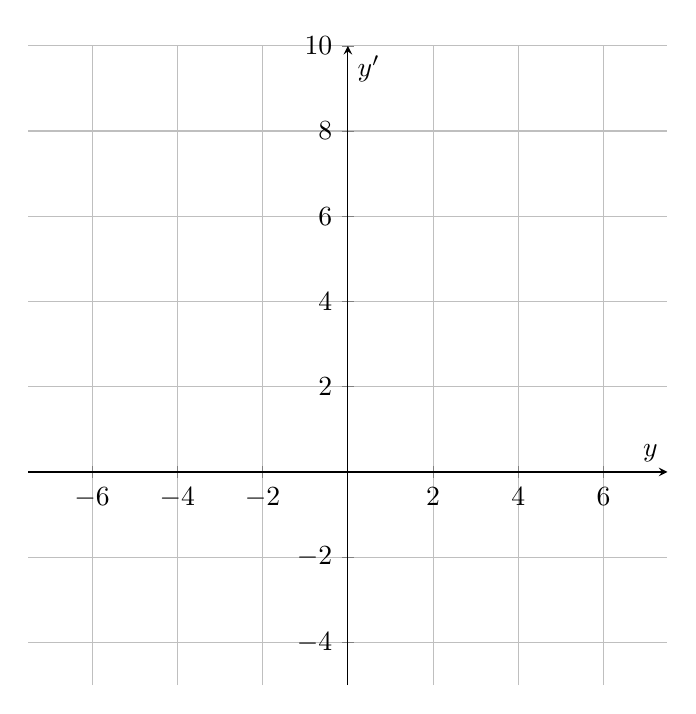
\begin{tikzpicture}
\begin{axis}[axis lines=center,axis equal,grid=both,
xmin=-4,xmax=4,ymin=-5,ymax=10,
width=0.8\textwidth,height=0.8\textwidth,
xlabel={$y$},
ylabel={$y'$}]
\end{axis}
\end{tikzpicture}

%\FloatBarrier
\begin{table}[H]
\caption{Sample table}
\label{table:disc}
\centering
\begin{tabular}{|l|l|l|l|}
\hline
Regime & $r$ & $\Delta_3(r)$ & Number of $\bar{y}$ \\ \hline
1      & -5  & 148           & 3                   \\ \hline
2      & 0   & -527          & 1                   \\ \hline
3      & 5   & 48            & 3                   \\ \hline
4      & 10  & -3741527      & 1                   \\ \hline
\end{tabular}
\end{table}
%\FloatBarrier
test1

\vspace{5mm}

test2


\begin{figure}[ht]
\centering
\includegraphics[scale=.65]{hw2_problem6b1.png}
\caption{Insert caption here.}
\label{fig:sample}
\end{figure}
\begin{lstlisting}
put pseudocode here
\end{lstlisting}
\end{comment}
\end{document}